\documentclass[aspectratio=169, 14pt]{beamer}
\usepackage[utf8]{inputenc}
\usepackage{xeCJK}
\usepackage{graphicx}
\usepackage{transparent}
\usepackage[ruled, lined, linesnumbered, commentsnumbered]{algorithm2e}
\usepackage{pgfplots}
\usepackage{tikz}
\usetikzlibrary{matrix,backgrounds}
\usetikzlibrary{arrows}
\usetikzlibrary {arrows.meta}
\usetikzlibrary{calc,shadows.blur,fit,positioning}
\usepackage{minted}
\usepackage{fontawesome5}
\usepackage{booktabs}
\usepackage{caption}
\usepackage{hyperref}
\hypersetup{
    colorlinks=true,
    linkcolor=blue,
    filecolor=magenta,      
    urlcolor=cyan,
    }
\urlstyle{same}
\usetheme{metropolis}
\metroset{block=fill}
\usecolortheme{default}
\definecolor{darkmidnightblue}{rgb}{0.0, 0.2, 0.4}
\definecolor{LightGray}{gray}{0.9}


%------------------------------------------------------------
%This block of code defines the information to appear in the
%Title page
\title[Database Principles and Applications] %optional
{数据库原理与应用}

\subtitle{SQL:修改数据库}

\author[CHEN Zhongpu] % (optional)
{CHEN Zhongpu}

\institute[] % (optional)
{
  School of Computing and Artificial Intelligence \\
  \href{mailto:zpchen@swufe.edu.cn}{zpchen@swufe.edu.cn}
}

\date[] % (optional)
{SWUFE, Spring \the\year{}}

%End of title page configuration block
%------------------------------------------------------------


%------------------------------------------------------------
%The next block of commands puts the table of contents at the 
%beginning of each section and highlights the current section:

% \AtBeginSection[]
% {
%   \begin{frame}
%     \frametitle{Table of Contents}
%     \tableofcontents[currentsection]
%   \end{frame}
% }
%------------------------------------------------------------


\begin{document}

%The next statement creates the title page.
\frame{\titlepage}

%---------------------------------------------------------
%This block of code is for the table of contents after
%the title page
% \begin{frame}
% \frametitle{Table of Contents}
% \tableofcontents
% \end{frame}
%--------------------------------------------------------
\begin{frame}
	\frametitle{复习}
	\begin{itemize}
		\item \texttt{select ... from ... where}
		\item \texttt{null}
		\item 聚集查询
		\item 嵌套子查询
	\end{itemize}
\end{frame}

\begin{frame}[fragile]
	\frametitle{小测试 (1)}

	\begin{columns}
		\column{.3\textwidth}
		\begin{table}
			\begin{tabular}{ll}
				\toprule
				name  & balance \\
				\midrule
				Bob   & 100     \\
				Alice & 50      \\
				Tom   & 50      \\
				Jack  & <null>  \\
				\bottomrule
			\end{tabular}
		\end{table}
		\column{.7\textwidth}
		给定右边的关系 \texttt{account (name, balance)},分析下面 SQL 查询的结果:

		\begin{minted}[bgcolor=LightGray]{sql} 
SELECT sum(balance) FROM account;

SELECT count(balance) FROM account;

SELECT count(*) FROM account;
    \end{minted}

	\end{columns}

\end{frame}

\begin{frame}
	\frametitle{小测试 (2)}
	考虑关系\texttt{instructor(ID, name, dept\_name, salary)},列出每个系老师的平均工资:

	\begin{enumerate}
		\item 使用 \texttt{group by} 子句
		\item 使用 标量子查询
	\end{enumerate}

\end{frame}

\begin{frame}[fragile]

	\begin{minted}[bgcolor=LightGray]{sql}
-- 方法1
SELECT dept_name, avg(salary)
FROM instructor
GROUP BY dept_name;

-- 方法2
SELECT dept_name,
    (SELECT avg(salary)
    FROM instructor
    WHERE instructor.dept_name = department.dept_name)
FROM department;
    \end{minted}

\end{frame}

{
% \usebackgroundtemplate{\transparent{0.3}{\begin{picture}
%     
\includegraphics[height=0.7\paperheight]{cover}
% \end{picture}    
% }}
\usebackgroundtemplate{
	\tikz[overlay,remember picture]
	\node[opacity=0.3, at=(current page.south east),anchor=south east, yshift=2cm,xshift=4cm] {
		
\includegraphics[height=0.6\paperheight]{cover}};
}
\begin{frame}
	\section{\textcolor{darkmidnightblue}{1. 增、删、改}}
\end{frame}

}

\begin{frame}[fragile]
	\frametitle{1.1 删除 (delete)}

	\begin{minted}[bgcolor=LightGray]{sql}
DELETE FROM r
WHERE p;
    \end{minted}

	\begin{minted}[bgcolor=LightGray, baselinestretch=1]{sql}
-- 删除 ID 是 8888 的教师
DELETE FROM instructor
WHERE ID = '8888';

-- 区别 drop 和 delete
DELETE FROM instructor;
DROP TABLE instructor;
    \end{minted}

\end{frame}

\begin{frame}
	\frametitle{练习 {\large \faIcon{code}} }
	\texttt{instructor(ID, name, dept\_name, salary)}

	\begin{enumerate}
		\item 删除工资在 70000 到 90000 之间的教师。
		\item 删除工资大于平均工资的教师。
	\end{enumerate}

\end{frame}

{\setbeamercolor{palette primary}{fg=black, bg=yellow}
\begin{frame}[standout]
	生产实践中一般并不会真的删除数据,而是将其设置为「不可见」。
\end{frame}
}

\begin{frame}[fragile]
	\frametitle{1.2 插入 (insert)}
	向 \texttt{course} 关系插入一条数据:

	\begin{minted}[bgcolor=LightGray, fontsize=\small]{sql}
-- 按属性列表次序(不推荐)
INSERT INTO course VALUES 
('CS-205', 'Database Systems', 'Comp. Sci.', 4);

-- 指定属性(可不按 DDL 的属性次序)
INSERT INTO course(course_id, title, dept_name, credits)
VALUES ('CS-205', 'Database Systems', 'Comp. Sci.', 4);
\end{minted}

\end{frame}

\begin{frame}[fragile]
	\frametitle{插入元组集合}
	\begin{minted}[bgcolor=LightGray]{sql}
-- 插入元组集合
INSERT INTO instructor VALUES 
('01', 'Bob', 'Music', 30000),
('02', 'Alice', 'Music', 30000);

-- 插入其他查询的结果
INSERT INTO instructor
SELECT ID, name, dept_name, 18000
FROM student
WHERE dept_name = 'Music' AND tot_cred > 144;
    \end{minted}

\end{frame}

\begin{frame}[fragile]
	\frametitle{插入部分属性}
	\begin{minted}[bgcolor=LightGray]{sql}
-- 剩下的属性取默认值或者 null
INSERT INTO instructor(id, name) VALUES 
('03', 'Mike');

INSERT INTO instructor VALUES 
('03', 'Mike', null, null);

-- PG 中的语法扩展
INSERT INTO instructor VALUES 
('03', 'Mike');
    \end{minted}
\end{frame}

\begin{frame}
	\frametitle{批量插入(导入)}

	{\Huge \faIcon{file} \faIcon{exchange-alt} \faIcon{database}}

	在 PG 中可以使用 \texttt{copy} 命令批量地从文件导入数据,执行速度比 \texttt{insert} 快得多,参考 \href{https://www.postgresql.org/docs/14/sql-copy.html}{COPY}。也可以直接在 DataGrip 中操作。

\end{frame}

\begin{frame}
	\frametitle{批量导出}
	导出到文件可以使用 \texttt{copy} 命令;也可以在 DataGrip 中操作。

	\begin{center}
		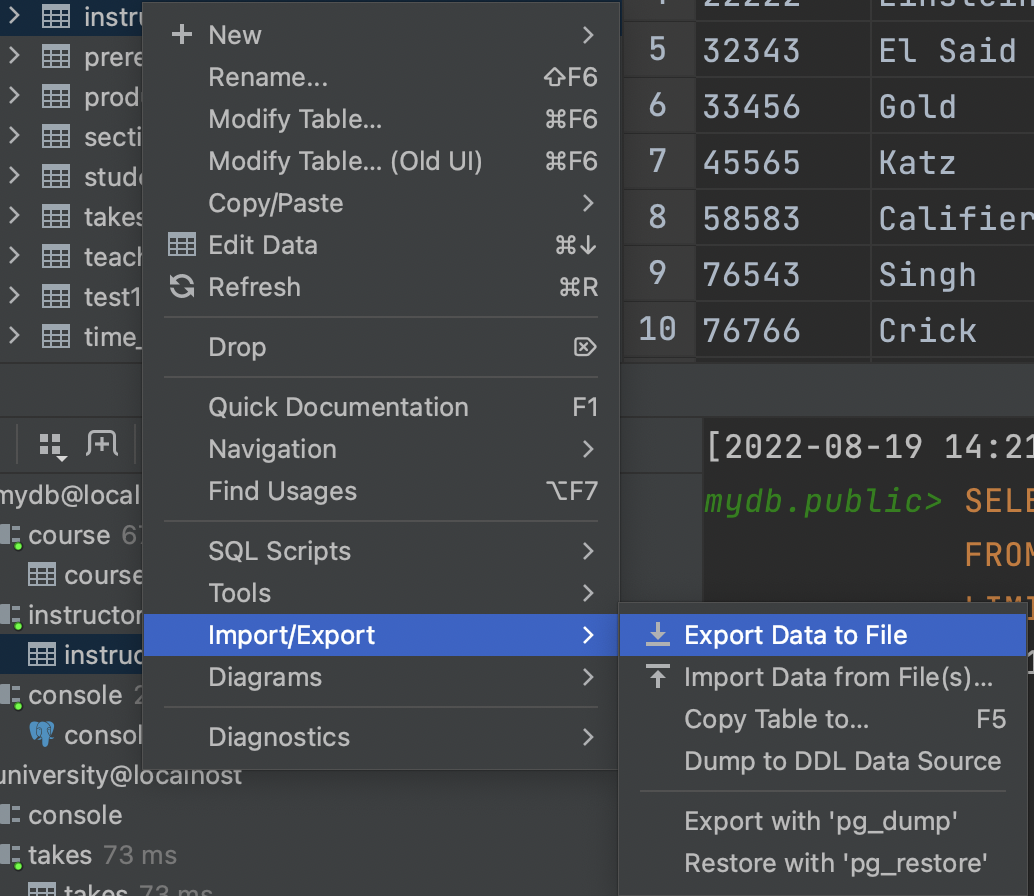
\includegraphics[height=.7\paperheight]{week6/export}
	\end{center}

\end{frame}

\begin{frame}[fragile]
	\frametitle{1.3 更新 (update)}

	\begin{minted}[bgcolor=LightGray]{sql}
-- 所有教师的工资增加 5%
UPDATE instructor
SET salary = salary * 1.05;

--- 仅对工资低于 70000 的教师涨工资
UPDATE instructor
SET salary = salary * 1.05
WHERE salary < 70000;
    \end{minted}

\end{frame}
\begin{frame}[fragile]
	\frametitle{update + case}

	给工资超过100000的老师涨3\%工资,其余老师涨5\%:

	\begin{minted}[bgcolor=LightGray]{sql}
UPDATE instructor
SET salary = CASE
    WHEN salary <= 100000 THEN salary * 1.05
    ELSE salary * 1.03
    END;
\end{minted}

	\begin{tikzpicture}
		\node[fill=yellow,blur shadow={shadow xshift=-0.5ex},
			text width=26em,anchor=south west,rounded corners]
		{如果分开更新,要注意次序;但 \texttt{case} 可以避免这个问题。};
	\end{tikzpicture}

\end{frame}

\begin{frame}
	\frametitle{练习}
	\href{https://www.w3school.com.cn/quiz/quiz.asp?quiz=sql}{W3School-SQL}
\end{frame}

\begin{frame}
	\frametitle{数据库的备份(自学)}
	PostgreSQL还提供了\texttt{pg\_dump}和\texttt{pg\_dumpall}等命令,用于数据库的备份与迁移。

	MySQL中也提供类似的命令,如{mysqldump}等。

	\begin{tikzpicture}
		\node[fill=yellow,blur shadow={shadow xshift=-0.5ex},
			text width=20em,anchor=south west,rounded corners]
		{这些命令是可执行程序,不是SQL命令。};
	\end{tikzpicture}

\end{frame}

\begin{frame}
	\frametitle{Homework 5}

	\href{https://github.com/ChenZhongPu/db-swufe/tree/master/06_sql}{06. SQL}

\end{frame}

\begin{frame}
	\section{\textcolor{darkmidnightblue}{2. DDL (2)}}
	修改关系 (\alert{alter table})
\end{frame}

\begin{frame}[fragile]
	\frametitle{2.1 新增属性}

	\begin{minted}[bgcolor=LightGray]{sql}
CREATE TABLE products (
    product_no integer,
    name text,
    price numeric
);
    \end{minted}

	使用 \alert{add column A D}:

	\begin{minted}[bgcolor=LightGray]{sql}
ALTER TABLE products ADD COLUMN description text;    
\end{minted}

\end{frame}

\begin{frame}[fragile]
	\frametitle{2.2 删除属性}
	使用 \alert{drop column A}:
	\begin{minted}[bgcolor=LightGray]{sql}
ALTER TABLE products DROP COLUMN description; 
    \end{minted}
	{\large \faIcon{code}}  \textbf{练习}:为关系 \texttt{student} 新增属性 \texttt{nationality},再删除它。

	\pause
	{\large \faIcon[regular]{lightbulb}}  \textbf{思考}:能否直接删除 \texttt{department} 的 \texttt{dept\_name}?

	\pause
	\begin{tikzpicture}
		\node[fill=yellow,blur shadow={shadow xshift=-0.5ex},
			text width=26em,anchor=south west,rounded corners]
		{如果属性被其他关系的外码引用,那么不能直接删除。};
	\end{tikzpicture}

	\begin{minted}[bgcolor=LightGray]{sql}
-- 级联删除
ALTER TABLE products DROP COLUMN description CASCADE;
\end{minted}

\end{frame}

\begin{frame}[fragile]
	\frametitle{2.3 其他修改}
	\begin{minted}[bgcolor=LightGray]{sql}
-- 修改属性的数据类型
ALTER TABLE products 
ALTER COLUMN price TYPE numeric(10,2);

-- 修改属性名
ALTER TABLE products 
RENAME COLUMN product_no TO product_number;

-- 修改关系名
ALTER TABLE products RENAME TO items;
    \end{minted}

\end{frame}

\begin{frame}
	\section{\textcolor{darkmidnightblue}{3. DDL (3)}}
	默认值、更多完整性约束

\end{frame}

\begin{frame}[fragile]
	\frametitle{3.1 默认值 (default)}
	如果没有显式地给出默认值,那么默认值就是 \texttt{null}。

	\begin{minted}[bgcolor=LightGray, baselinestretch=1]{sql}
CREATE TABLE products (
    product_no integer,
    name text,
    price numeric DEFAULT 9.99
);
\end{minted}

\end{frame}

\begin{frame}[fragile]
	默认值可以在 \texttt{insert} 命令中被使用:

	\begin{minted}[bgcolor=LightGray, baselinestretch=1]{sql}
INSERT into products (product_no, name) VALUES
(88, 'Apple');
    \end{minted}

	甚至可以在 \texttt{insert} 中直接使用 \texttt{default}:

	\begin{minted}[bgcolor=LightGray, baselinestretch=1]{sql}
INSERT into products VALUES
(88, 'Apple', DEFAULT);
\end{minted}

\end{frame}

\begin{frame}[fragile]
	\frametitle{修改默认值}

	\begin{minted}[bgcolor=LightGray, baselinestretch=1]{sql}
ALTER TABLE products 
ALTER COLUMN price SET DEFAULT 8.88;

-- 清除默认值
ALTER TABLE products 
ALTER COLUMN price DROP DEFAULT;
    \end{minted}

\end{frame}

\begin{frame}[fragile]
	\frametitle{3.2 unique}

	\begin{quote}
		\textbf{完整性约束}保证用户对数据库所做的修改不会破坏数据的一致性。
	\end{quote}

	\begin{itemize}
		\item \texttt{primary key}
		\item \texttt{not null}
		\item \texttt{foreign key}
	\end{itemize}
	\pause

	\begin{minted}[bgcolor=LightGray]{sql}
-- 通过修改关系添加约束
ALTER TABLE products 
ADD CONSTRAINT some_name UNIQUE (product_no);
\end{minted}

\end{frame}

\begin{frame}[fragile]

	\begin{minted}[bgcolor=LightGray, baselinestretch=.9]{sql}
CREATE TABLE products (
    product_no integer UNIQUE, -- 行约束
    name text,
    price numeric
);

CREATE TABLE products (
    product_no integer,
    name text,
    price numeric,
    UNIQUE (product_no) -- 表约束
);
    \end{minted}

	{\large \faIcon{code}}  \textbf{练习}:有 \texttt{unique} 约束的值能否为 \texttt{null}?

\end{frame}

{\setbeamercolor{palette primary}{fg=black, bg=yellow}
\begin{frame}[standout]
	\texttt{primary key} 大致相当于 \texttt{not null} 加上 \texttt{unique}。
\end{frame}
}

\begin{frame}[fragile]
	\frametitle{3.3 check}
	\texttt{check} 约束最通用。\texttt{check(P)} 子句指定一个谓词,关系中的每个元组都必须满足 \texttt{P}。

	\begin{minted}[bgcolor=LightGray]{sql}
-- 也可以写成表约束
CREATE TABLE products (
    product_no integer,
    name text,
    price numeric CHECK (price > 0)
);
\end{minted}

\end{frame}

\begin{frame}[fragile]

	\begin{minted}[bgcolor=LightGray]{sql}
CREATE TABLE products (
    product_no integer,
    name text,
    price numeric,
    CHECK (price > 0),
    discounted_price numeric,
    CHECK (discounted_price > 0),
    CHECK (price > discounted_price)
);
    \end{minted}
\end{frame}

\begin{frame}[fragile]
	\begin{minted}[bgcolor=LightGray]{sql}
CREATE TABLE products (
    product_no integer,
    name text,
    price numeric CHECK (price > 0)
);
    \end{minted}
	{\large \faIcon{code}}  \textbf{练习}:\texttt{price} 能否为空?

	\pause

	\begin{tikzpicture}
		\node[fill=yellow,blur shadow={shadow xshift=-0.5ex},
			text width=26em,anchor=south west,rounded corners]
		{\texttt{check}需要满足的条件是 \textbf{not false}。因此,允许出现 \texttt{null},即 \texttt{unknown}。};
	\end{tikzpicture}

\end{frame}

\begin{frame}[fragile]
	\frametitle{例子}

	\begin{minted}[bgcolor=LightGray, baselinestretch=.9, fontsize=\small]{sql}
CREATE TABLE section1 (
    course_id    varchar(8),
    sec_id       varchar(8),
    semester     varchar(6),
    year         numeric(4, 0),
    building     varchar(15),
    room_number  varchar(7),
    time_slot_id varchar(4),
    primary key (course_id, sec_id, semester, year)
);
\end{minted}

	考虑添加约束:\texttt{semester} 只能是 \texttt{Spring} 或 \texttt{Fall};\texttt{year} 在 1976 到 2100 之间;\texttt{course\_id} 为外码,参照关系 \texttt{course}。
\end{frame}

\begin{frame}[fragile]
	\frametitle{资料}
	SQL 还支持对 \texttt{unique} 和 \texttt{check} 约束进行命名,参考 \href{https://www.postgresql.org/docs/14/ddl-constraints.html}{Constraints}。

	\begin{minted}[bgcolor=LightGray, fontsize=\small]{sql}
CREATE TABLE products (
    product_no integer,
    name text,
    price numeric,
    CHECK (price > 0),
    discounted_price numeric,
    CHECK (discounted_price > 0),
    CONSTRAINT valid_discount CHECK (price > discounted_price)
);
\end{minted}

\end{frame}

\begin{frame}[fragile]
	\frametitle{3.4 再谈外码}
	关系\texttt{section}中的\texttt{course\_id} 为外码,参照关系 \texttt{course},那么能否直接将\texttt{course}中某门课程删除?

	\begin{minted}[bgcolor=LightGray,]{sql}
INSERT INTO course
VALUES ('CS-600', 'Advanced DB', 'Comp. Sci.', 4);

INSERT INTO section1 VALUES ('CS-600', '1', 'Spring', 
2022, 'Watson', '100', 'A');

DELETE FROM course
WHERE course_id = 'CS-600';
\end{minted}

\end{frame}

\begin{frame}
	删除外码所引用的元组时,有四种可能的行为:
	\begin{itemize}
		\item(默认)禁止删除
		\item \texttt{ON DELETE CASCADE}
		\item \texttt{ON DELETE SET NULL}
		\item \texttt{ON DELETE SET DEFAULT}
	\end{itemize}

	不难发现,\texttt{UPDATE}命令也是类似的。

\end{frame}

\begin{frame}
	\section{\textcolor{darkmidnightblue}{4. SQL排名}}

	\begin{table}
		\caption*{2021年双11京东手机销量排行}
		\begin{tabular}{ll}
			\toprule
			型号         & 排名 \\
			\midrule
			iPhone 13  & 1  \\
			Redmi K 40 & 2  \\
			iPhone 12  & 3  \\
			\bottomrule
		\end{tabular}
	\end{table}
\end{frame}

\begin{frame}[fragile]
	\frametitle{4.1 RANK}

	\begin{minted}[bgcolor=LightGray,]{sql}
SELECT id, salary FROM instructor
ORDER BY salary DESC;

SELECT id, salary, 
       RANK() OVER (ORDER BY (salary) DESC) as s_rank
FROM instructor
ORDER BY s_rank;
    \end{minted}

	\pause
	\begin{tikzpicture}
		\node[fill=yellow,blur shadow={shadow xshift=-0.5ex},
			text width=20em,anchor=south west,rounded corners]
		{ORDER BY降序时会把NULL排在最前面。};
	\end{tikzpicture}

\end{frame}

\begin{frame}[fragile]

	有多种方案:
	\begin{minted}[bgcolor=LightGray,]{sql}
-- 排除NULL
SELECT salary FROM instructor
WHERE salary IS NOT NULL
ORDER BY salary DESC;

-- 将NULL放在最后面
SELECT id, salary FROM instructor
ORDER BY salary DESC NULLS LAST;
\end{minted}

\end{frame}

\begin{frame}[fragile]
	\frametitle{回顾}
	\begin{exampleblock}{Homework 4}
		找到工资最高的员工(可能不唯一)。
	\end{exampleblock}

	\begin{minted}[bgcolor=LightGray,]{sql}
-- 是否正确?
SELECT id FROM instructor
ORDER BY salary DESC
LIMIT 1;
\end{minted}

\end{frame}

\begin{frame}[fragile]

	\begin{minted}[bgcolor=LightGray, fontsize=\small]{sql}
-- 是否正确?
SELECT id,
RANK() OVER (ORDER BY salary DESC NULLS LAST) AS s_rank
FROM instructor
WHERE s_rank = 1;
    \end{minted}

	\pause
	\begin{tikzpicture}
		\node[fill=yellow,blur shadow={shadow xshift=-0.5ex},
			text width=24em,anchor=south west,rounded corners]
		{SELECT子句的alias不能用于WHERE子句!};
	\end{tikzpicture}

	\begin{minted}[bgcolor=LightGray]{sql}
-- 不合法!
SELECT id, salary/12 AS m_salary
FROM instructor
WHERE m_salary > 5000;
    \end{minted}

\end{frame}

\begin{frame}[fragile]

	\begin{minted}[bgcolor=LightGray, fontsize=\small]{sql}
SELECT id FROM 
   (SELECT id, 
   RANK() OVER (ORDER BY salary DESC NULLS LAST) AS s_rank
   FROM instructor) AS a
WHERE s_rank = 1;
    \end{minted}


\end{frame}
\end{document}
